\documentclass{article}

\usepackage[german]{babel}
\usepackage{array}
\usepackage[letterpaper,top=2cm,bottom=2cm,left=3cm,right=3cm,marginparwidth=1.75cm]{geometry}

\usepackage{amsmath}
\usepackage{graphicx}
\usepackage{subcaption} % Added package
\usepackage[colorlinks=true, allcolors=blue]{hyperref}
\usepackage[T1]{fontenc}
\usepackage{tabularx}
\usepackage{booktabs}


\title{Übungsprotokoll - NWG2 - Übung 04 \\ VLANS}
\author{\vspace{0.5cm} Thomas Brandstetter (s2210239002) \& Jakob Mayr (s2210239021)}

\begin{document}
\maketitle

\section{Konfiguration der Endsysteme}

In der folgenden Übung haben wir die PCs 4.1 und 4.2 benutzt, somit sind die Netze 4.x verwendet worden. Die IP-Konfiguration wird folgendermaßen vergeben: Klick auf „Network“ in der Taskleiste $\rightarrow$ „Network \& Internet Settings“ $\rightarrow$ „Change adapter options“ $\rightarrow$ gewünschtes Netzwerk Interface auswählen, in diesem Fall Ethernet 2 $\rightarrow$ „Properties“ $\rightarrow$ Doppelklick auf „Internet Protocol Version 4“ bzw. „Internet Protocol Version 6“. In den geöffneten Fenstern können wir nun jeweils die IP-Adresse, Subnetzmaske/Präfix und das Gateway eingeben. Folglich sind die Konfigurationen beider PCs zu sehen:

\begin{figure}[!htp]
  \centering
  \begin{minipage}[b]{0.2\textwidth}
    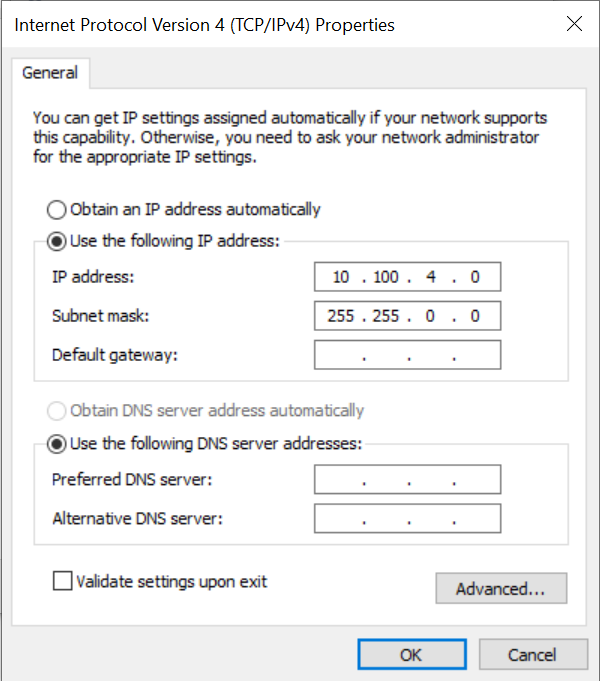
\includegraphics[width=\textwidth]{Arbeitsergebnisse/PC41/pc41_IPv4_config.png}
    \caption{PC41 IPv4 config}
  \end{minipage}
  \hspace{0.8cm}
  \begin{minipage}[b]{0.2\textwidth}
    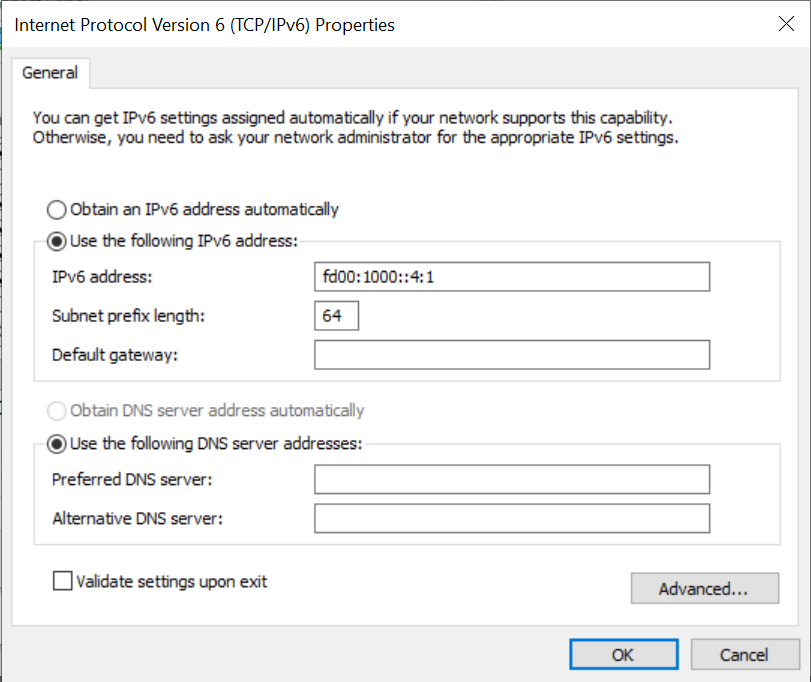
\includegraphics[width=\textwidth]{Arbeitsergebnisse/PC41/pc41_IPv6_config.png}
    \caption{PC41 IPv6 config}
  \end{minipage}
  \hspace{0.8cm}
  \begin{minipage}[b]{0.2\textwidth}
    \includegraphics[width=\textwidth]{Arbeitsergebnisse/PC42/pc42_IPv4_config.png}
    \caption{PC42 IPv4 config}
  \end{minipage}
  \hspace{0.8cm}
  \begin{minipage}[b]{0.2\textwidth}
    \includegraphics[width=\textwidth]{Arbeitsergebnisse/PC42/pc42_IPv6_config.png}
    \caption{PC42 IPv6 config}
  \end{minipage}
\end{figure}

\pagebreak
\section{Konfiguration des Gruppenswitches}

Für die Konfiguration des Gruppenswitches wurden für die Clients die Ports FastEthernet0/11 und FastEthernet0/12, für den Backbone-Switch der Port GigabitEthernet0/1 und für den Gruppenrouter der Port GigabitEthernet0/2 verwendet.
Die Ports für die Clients wurden mit dem „access mode“ für die VLANS 41 bzw. 42 konfiguriert.

\begin{table}[htbp]
    \centering
    \begin{tabularx}{\textwidth}{|X|X|}
        \toprule
        \textbf{Befehl} & \textbf{Erklärung} \\
        \midrule
        switchport access vlan <vlan-tag-numbers> & Mit diesem Befehl wird ein Switchport im „access mode“ einem oder mehreren VLANS zugeordnet.\\
        \hline
        switchport mode access & Mit diesem Befehl wird ein switchport in den „access mode“ gesetzt.\\
        \bottomrule
    \end{tabularx}
    \caption{Verwendete Befehle der Switchports für die Clients}
    \label{tab:commands}
\end{table}
\noindent Die Ports für den Backbone-Switch und den Gruppenrouter wurden mit dem „trunk mode“ konfiguriert und haben daher keine zugehörige VLAN-Konfiguration.

\begin{table}[htbp]
    \centering
    \begin{tabularx}{\textwidth}{|X|X|}
        \toprule
        \textbf{Befehl} & \textbf{Erklärung} \\
        \midrule
        switchport mode trunk & Mit diesem Befehl wird ein switchport in den „trunk mode“ gesetzt.\\
        \hline
         switchport trunk allowed vlan <vlan-tag-numbers> & Mit diesem Befehl wird ein switchport im „trunk mode“ einem oder mehreren VLANS zugeordnet.\\
        \bottomrule
    \end{tabularx}
    \caption{Verwendete Befehle der Switchports für Backbone und Router}
\end{table}

\section{Konfiguration des Gruppenrouters}

Für die Konfiguration des Gruppenrouters wurde der Port GigabitEthernet0/0 verwendet. Da das Interface pro VLAN eine unterschiedliche Adressen + Masken benötigt, werden hierfür Subinterfaces (virtuelle Interfaces) verwendet. Das Subinterface GigabitEthernet0/0.42 wird dem VLAN 42 und das Subinterface GigabitEthernet0/0.45 dem VLAN 45 zugewiesen. Zudem muss auf dem Router eine Default-Route zum Backbone-Router konfiguriert werden.

\begin{table}[htbp]
    \centering
    \begin{tabularx}{\textwidth}{|X|X|}
        \toprule
        \textbf{Befehl} & \textbf{Erklärung} \\
        \midrule
        encapsulation dot1Q <vlan-tag-number> & Mit diesem Befehl wird ein Interface einem VLAN zugewiesen.\\
        \hline
        ip address <ip-address> <ip-address-mask> & Mit diesem Befehl wird einem dem ausgewählten Interface eine IPv4-Adresse und Maske zugewiesen.\\
        \hline
        ipv6 address <ip-address/ip-address-mask> & Mit diesem Befehl wird einem dem ausgewählten Interface eine IPv6-Adresse und Maske zugewiesen.\\
        \hline
        ip <routenetwork-number> <network-mask> <ip-address> | interface> & Mit diesem Befehl wird eine statische IPv4 Route in der Routing-Tabelle angelegt.\\
        \hline
        ipv6 <routenetwork-number/network-mask> <ip-address | interface> & Mit diesem Befehl wird eine statische IPv6 Route in der Routing-Tabelle angelegt.\\
        \bottomrule
    \end{tabularx}
    \caption{Verwendete Befehle für die Konfiguration des Gruppenrouters}
    \label{tab:commands}
\end{table}
\noindent Bei der Konfiguration des Gruppenrouters müssen natürlich wieder das ipv6-unicast-routing (mit dem bereits bekannten Befehl) und der Befehl „no shutdown“ für das Interface verwendet werden.

\section{Fragen zur Konfiguration}

\subsection*{Frage 4.1 \normalfont Warum sind verschiedene VLANs im selben IP Netz nicht sinnvoll?}
Es ergeben sich folgende Probleme:
\begin{itemize}
\item Da alle VLANs denselben IP-Bereich verwenden, kann es zu IP-Adresskonflikten kommen. Zwei oder mehr Geräte auf verschiedenen VLANs könnten versuchen, dieselbe IP-Adresse zu verwenden, was zu Konflikten und Kommunikationsproblemen führt.
\item Wenn alle VLANs denselben IP-Bereich verwenden, kann es schwierig sein, Netzwerkprobleme zu diagnostizieren und zu beheben. Da die IP-Adressen nicht eindeutig sind, kann es schwierig sein, festzustellen, welche Geräte Probleme verursachen oder welche Geräte betroffen sind.
\end{itemize}
Insgesamt ist es empfehlenswert, VLANs und IP-Netzwerke getrennt voneinander zu planen und zu konfigurieren, um eine klare Segmentierung, bessere Kontrolle und Sicherheit im Netzwerk zu gewährleisten.


\subsection*{Frage 4.2 \normalfont Warum müssen auf den Subinterfaces die VLANs bekannt gegeben werden? Warum muss der angeschlossene Switch Port ein Trunk Port sein?}
Die VLAN-IDs müssen auf den Subinterfaces bekannt gegeben werden, 
um den Datenverkehr zu kennzeichnen, der über ein spezifisches VLAN fließen soll. Jedes Subinterface wird in der Regel mit einer bestimmten VLAN-ID konfiguriert, was dem Router ermöglicht, den Datenverkehr
 basierend auf diesen VLAN-IDs zu unterscheiden und korrekt zu routen. Standardmäßig würde ein Port im „trunk mode“ alle VLANs routen, da die Aufgabenstellung allerdings verlangt, dass nur bestimmte VLANs geroutet werden können, müssen diese explizit angegeben werden.\\
Ein Trunk Port wird benötigt, damit über diesen Port Netzwerkverkehr von mehreren VLANs geroutet werden können.

\subsection*{Frage 4.3 \normalfont Könnte eine Anbindung der Gruppenrouter auch ohne Subinterfaces funktionieren? Wenn ja, wie?}
Man könnte alternativ auch für jedes VLAN ein eigenes Interface verwenden, da ein Router allerdings eine begrenzte Anzahl von Ports hat, ist dies nicht sinnvoll.

\subsection*{Frage 4.4 \normalfont Warum ist hier das anlegen der Default Routen nötig? Welche Erreichbarkeiten sind nur so sicherzustellen.}
Um beispielsweise von dem Client PC42 auf den next-hop, in diesem Fall der Backbone Router, zu kommen müssen Default-Routen angelegt werden. Der Client hat als Gateway den GR41 (Gruppenrouter) angegeben und muss somit von diesem weitergeroutet werden.


\subsection*{Frage 4.5 \normalfont Wie wirken sich Trunk Ports auf die Source Address Table aus? Warum ändert sich die Source Address Table im Lauf der Zeit?}
Da über Trunk Ports mehrer MAC-Addressen angeschlossen sind entstehen im Source Address Table pro Port auch mehrere Einträge. Da mit der Zeit durch ARP-Requests weitere Adressen „gelernt“ werden erweitert sich die Tabelle.

\pagebreak
\section{Tests und Interpretation ihrer Resultate}

\subsection{GR41}
Ping von Gruppenrouter 41 zum Backbone Router sowie die Routing Tabelle des Gruppenrouters.\\
\begin{figure}[!htp]
  \centering
  \begin{minipage}[b]{0.45\textwidth}
    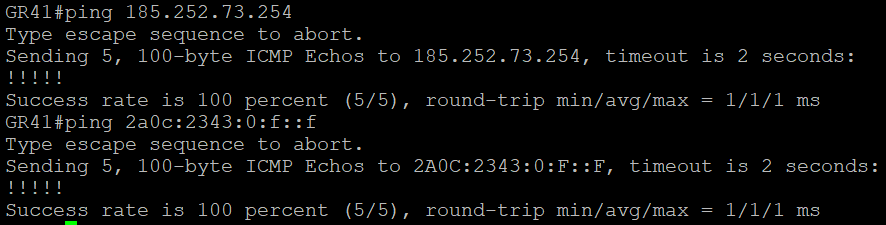
\includegraphics[width=\textwidth]{Arbeitsergebnisse/GR41/gr41_ping_backbone.png}
    \caption{GR41 ping backbone}
  \end{minipage}
  \hspace{0.8cm}
  \begin{minipage}[b]{0.45\textwidth}
    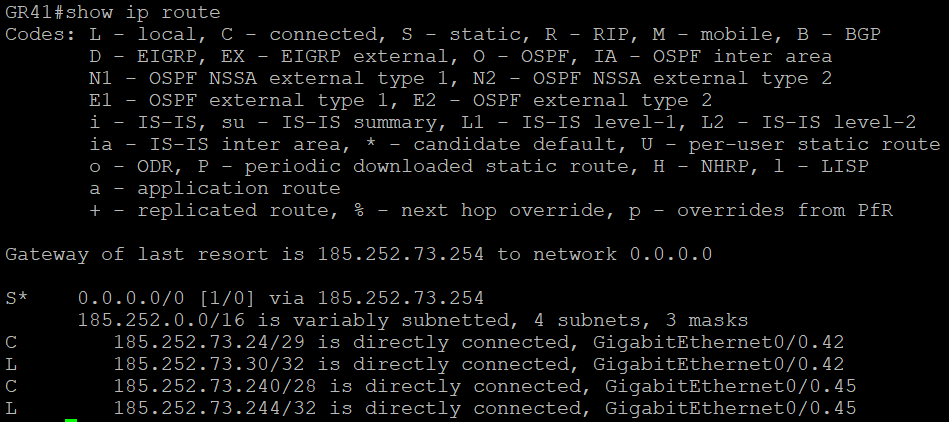
\includegraphics[width=\textwidth]{Arbeitsergebnisse/GR41/gr41_routing_table.png}
    \caption{GR41 routing table}
  \end{minipage}
\end{figure}

\subsection{GS41}
Source (oder MAC) Address Tabelle des Gruppenswitches.\\
\begin{figure}[!htp]
  \centering
  \begin{minipage}[b]{0.45\textwidth}
    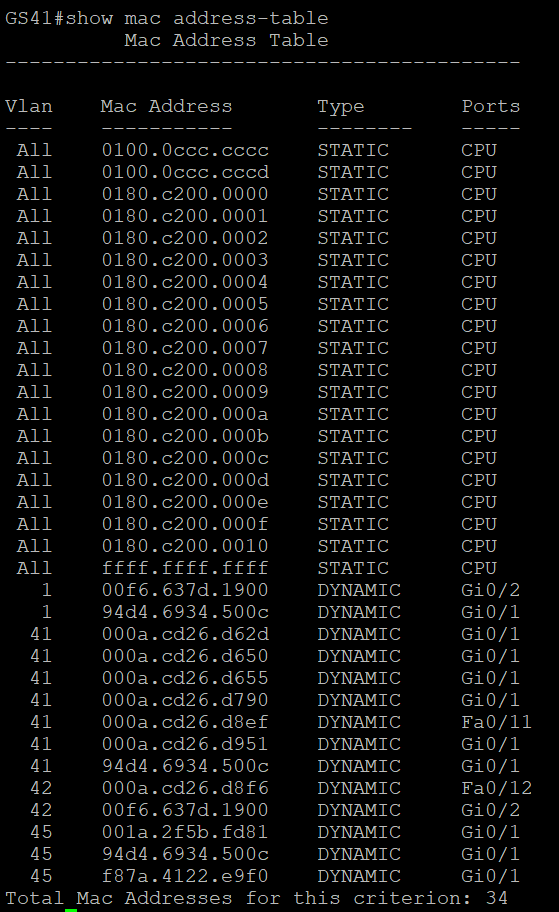
\includegraphics[width=\textwidth]{Arbeitsergebnisse/GS41/gs41_mac_address-table.png}
    \caption{GS41 mac address table}
  \end{minipage}
\end{figure}

\pagebreak
\subsection{PC41}
Ping von PC41 zu PC0, Ping von PC41 zu PC31 in Netz 3 sowie Ping von PC41 zu PC61 in Netz 6.\\
\begin{figure}[!htp]
  \centering
  \begin{minipage}[b]{0.25\textwidth}
    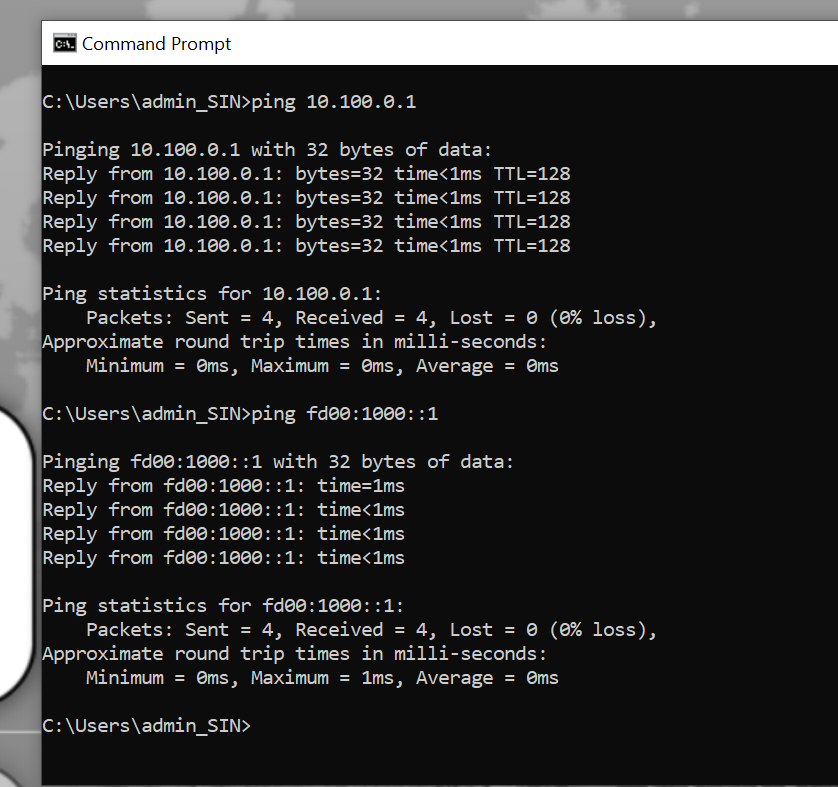
\includegraphics[width=\textwidth]{Arbeitsergebnisse/PC41/pc41_ping_pc0.png}
    \caption{PC41 ping PC0}
  \end{minipage}
  \hspace{0.8cm}
  \begin{minipage}[b]{0.25\textwidth}
    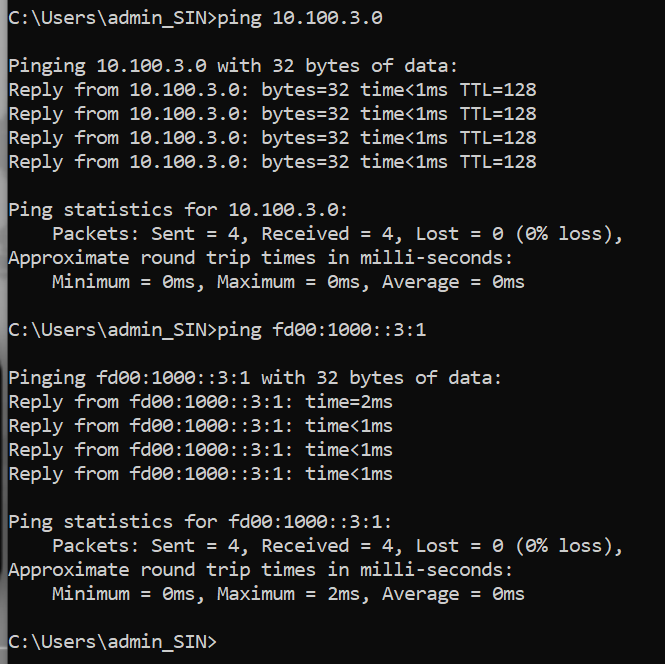
\includegraphics[width=\textwidth]{Arbeitsergebnisse/PC41/pc41_ping_net3.png}
    \caption{PC41 ping Netz3}
  \end{minipage}
  \hspace{0.8cm}
  \begin{minipage}[b]{0.25\textwidth}
    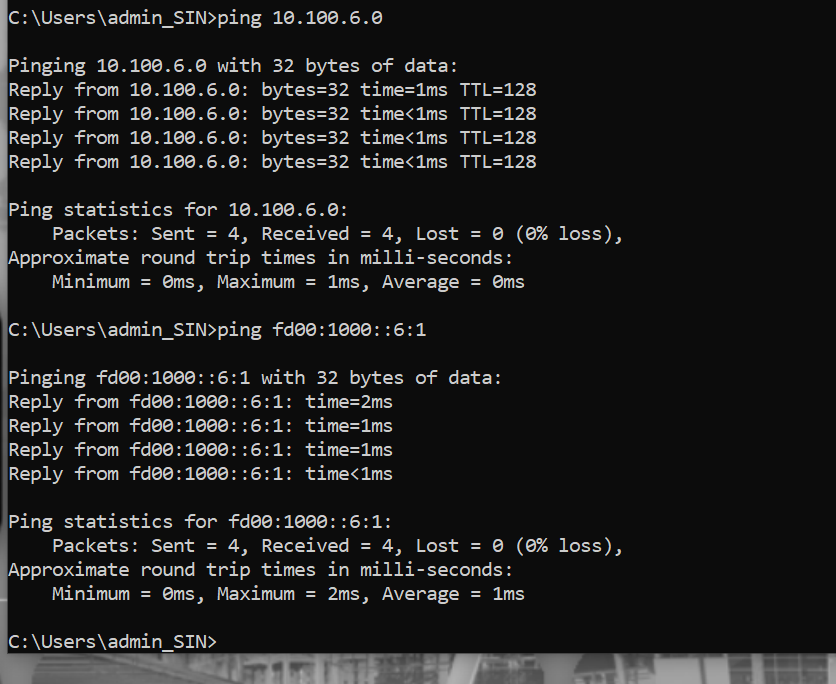
\includegraphics[width=\textwidth]{Arbeitsergebnisse/PC41/pc41_ping_net6.png}
    \caption{PC41 ping Netz6}
  \end{minipage}
\end{figure}

\subsection{PC42}
Ping von PC42 zum Backbone Router, Ping von PC41 zum GR41, Ping von PC42 zu PC32 in Netz 3 sowie Ping von PC42 zu PC52 in Netz 5.\\
\begin{figure}[!htp]
  \centering
  \begin{minipage}[b]{0.2\textwidth}
    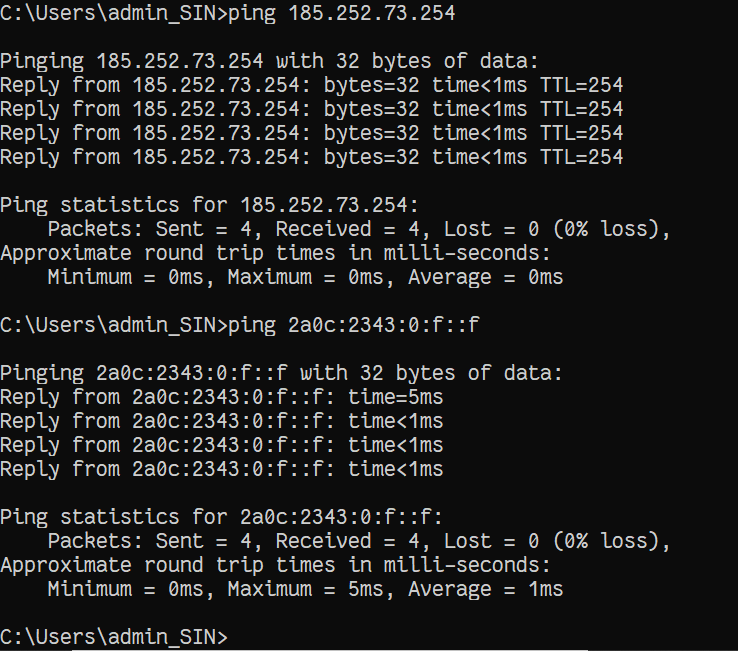
\includegraphics[width=\textwidth]{Arbeitsergebnisse/PC42/pc42_ping_backbone.png}
    \caption{PC42 ping backbone}
  \end{minipage}
  \hspace{0.8cm}
  \begin{minipage}[b]{0.2\textwidth}
    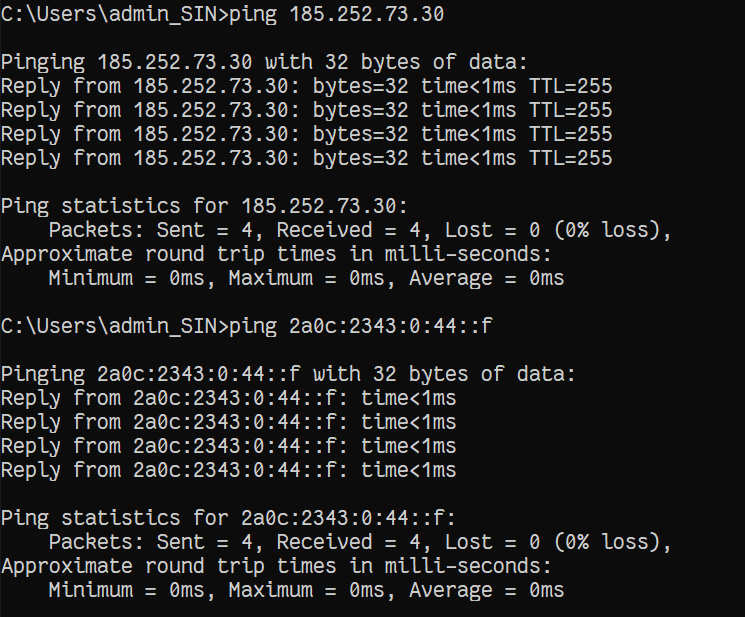
\includegraphics[width=\textwidth]{Arbeitsergebnisse/PC42/pc42_ping_gr41.png}
    \caption{PC42 ping gr41}
  \end{minipage}
  \hspace{0.8cm}
  \begin{minipage}[b]{0.2\textwidth}
    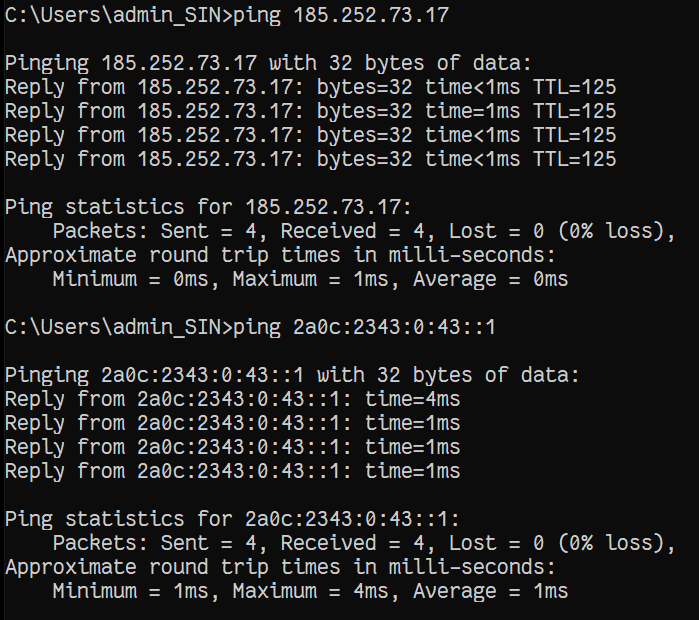
\includegraphics[width=\textwidth]{Arbeitsergebnisse/PC42/pc42_ping_net3.png}
    \caption{PC42 ping Netz3}
  \end{minipage}
  \hspace{0.8cm}
  \begin{minipage}[b]{0.2\textwidth}
    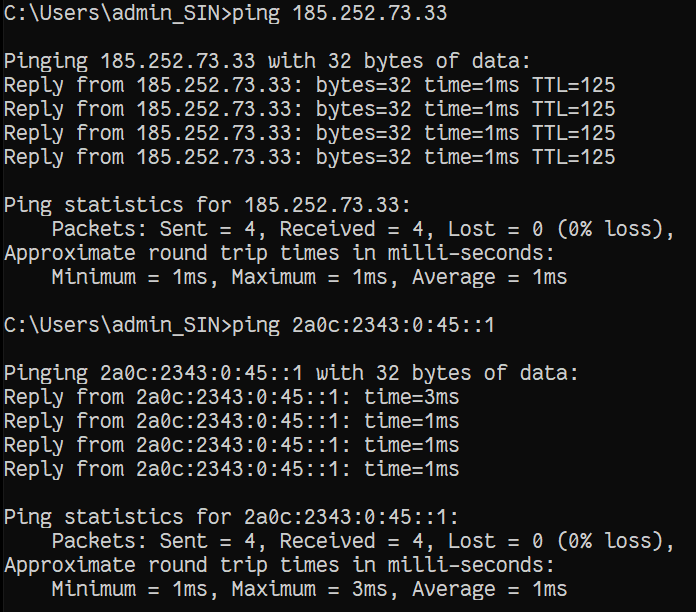
\includegraphics[width=\textwidth]{Arbeitsergebnisse/PC42/pc42_ping_net5.png}
    \caption{PC42 ping Netz5}
  \end{minipage}
\end{figure}

\end{document}

